%present.tex, Dan Richardson

\documentclass{beamer}
\mode<presentation>

\usepackage{graphicx}                  %use package for diagram 
\usepackage{amsmath}                   %use package for implies symbol
\usepackage{amsfonts}		       %use package for numbet sets
\usepackage{bm}                        %use package for bolds in math mode
\usepackage{tikz}                      %use package for diagram drawings
\usepackage{algpseudocode}             %use package for pseudocode
\usepackage{algorithm}                 %use package for pseudocode
\usepackage{caption}                   %use package for multiple figures
\usepackage{subcaption}                %use package for multiple figures
%\usepackage{listings}                  %use package for c++ code in appendix
%\usepackage{colour}                    %use package for code listings
%\usepackage[utf8]{inputenc}            %use package for colours in code
%\usepackage{url}                       %use package to display urls properly
%\usepackage{array}                     %use package for centering table contents

%define colours for code listings
%\definecolor{codegreen}{rgb}{0,0.6,0}
%\definecolor{codegray}{rgb}{0.5,0.5,0.5}
%\definecolor{codepurple}{rgb}{0.58,0,0.82}
%\definecolor{backcolour}{rgb}{0.95,0.95,0.92}

%define a style for the listings
%\lstdefinestyle{mystyle}{
%    backgroundcolor=\color{backcolour},
%    commentstyle=\color{codegreen},
%    keywordstyle=\color{magenta},
%    numberstyle=\tiny\color{codegray},
%    stringstyle=\color{codepurple},
%    basicstyle=\footnotesize,
%    breakatwhitespace=false,
%    breaklines=true,
%    captionpos=b,
%    keepspaces=true,
%    numbers=left,
%    numbersep=5pt,
%    showspaces=false,
%    showstringspaces=false,
%    showtabs=false,
%    tabsize=2
%}

%set style of listing to that defined above
%\lstset{style=mystyle}

%set style of footnotes
%\renewcommand{\thefootnote}{\roman{footnote}}

%define command shortcuts
\newcommand{\be}{\begin{equation}}
\newcommand{\ee}{\end{equation}}

%use tikz library for shapes
\usetikzlibrary{shapes.geometric, arrows}

%define block styles in tikz
\tikzstyle{startstop} = [rectangle, rounded corners, minimum width=3cm, minimum height=1cm, text centered, draw=black, fill=red!30]
\tikzstyle{io} = [trapezium, trapezium left angle=70, trapezium right angle=110, minimum width=3cm, minimum height=1cm, text centered, draw=black, fill=blue!30]
\tikzstyle{process} = [rectangle, minimum width=3cm, minimum height=1cm, text centered, draw=black, fill=orange!30]
\tikzstyle{decision} = [diamond, minimum width=3cm, minimum height=1cm, text centered, draw=black, fill=green!30]
\tikzstyle{arrow} = [thick,->,>=stealth]

%set graphics path
\graphicspath{{/home/danmfr/p3t/laplace/images/}}

\title{On the effect of solid conductors on the electric field}
\author{S. Brown, F. Hayes, L. Heikkil{\"a}, W. Liu, D. Richardson\\
        School of Physics and Astronomy,\\
        University of Glasgow,\\
        Glasgow, United Kingdom}
\date{\today}

\AtBeginSection[] %layout page at start of new section
{
  \begin{frame}<beamer>
    \frametitle{Layout}
    \tableofcontents[currentsection,currentsubsection]
  \end{frame}
}

\begin{document} %start of document

\begin{frame} 
\titlepage
\end{frame}

\section{Introduction}

\begin{frame}{Electrostatic Systems}

\begin{figure}
\centering
\begin{subfigure}[b]{0.45\textwidth}
	\begin{tikzpicture}
	\draw (0,0) -- (0,2.5) node[above, font=\footnotesize] {$\phi = V$}; 
	\draw (4.2,0) -- (4.2,2.5) node[above, font=\footnotesize] {$\phi = -V$}; 
	\draw (2.1,1.25) circle (0.5cm) node[below, font=\footnotesize, yshift=-0.4cm] {GND};
	\draw[dashed] (2.1,1.25) -- (2.5,1.55) node[pos=0.2, above, font=\footnotesize] {$R$};
	\end{tikzpicture}
	\caption{System A}
\end{subfigure}
\hfill
\begin{subfigure}[b]{0.45\textwidth}
	\begin{tikzpicture}
	\draw (0,0) -- (4,0) node[right, font=\footnotesize] {$\phi = V$}; 
	\draw (0,2.5) -- (4,2.5) node[pos=0.25, above, font=\footnotesize] {GND} node[pos=0.5, above, font=\footnotesize] {GND} node[pos=0.75,above, font=\footnotesize] {GND};
	\draw (0.8,2.5) rectangle (1.2,2.375);
	\draw (1.8,2.5) rectangle (2.2,2.375);
	\draw (2.8,2.5) rectangle (3.2,2.375);
	\end{tikzpicture}
	\caption{System C}
\end{subfigure}
\caption{Cross-sectional diagram of two electrostatic systems}
\end{figure}

\end{frame}

\begin{frame}{Derivation of Laplace's Equation}
We have two of Maxwell's equations
%
\be
\nabla \cdot \bm{E} = \frac{Q}{\epsilon_0} \qquad \nabla \times \bm{E} = -\frac{\partial \bm{B}}{\partial t}
\ee

In both systems:
\begin{itemize}
\item $\bm{B}$ is unchanging $\implies$ $\bm{E}$ is irrotational $\implies \bm{E} = -\nabla \phi$
\item $Q=0$ $\implies \bm{E}$ is solenoidal $\implies \nabla^2 \phi = 0$.
\end{itemize}

This is Laplace's equation.
\end{frame}

\section{Analytical Solution}

\begin{frame}{General Solution}
Wish to solve $\nabla ^2 \phi = 0$ in polar co-ordinates:
%
\be
\frac{1}{r}\frac{\partial}{\partial r}(r \frac{\partial \phi}{\partial r})
+ \frac{1}{r^2}\frac{\partial ^2 \phi}{\partial \theta^2} = 0
\ee

Separate variables, $\phi(r,\theta)=f(r)g(\theta)$, say.

Produces pair of second-order ODEs, for some $k \in \mathbb{R}$:
%
\be
r\frac{d}{dr}(r \frac{df(r)}{dr}) = k^2 f(r) \quad \frac{d^2 g(\theta)}{d\theta^2} = -k^2 g(\theta)
\ee

Solve to give general solution in polar co-ordinates:
%
\begin{multline}
\phi(r, \theta) = (\alpha_0 \ln(r) + \beta_0)(\gamma_0\theta + \delta_0) + 
\\
                + \sum_{n=1}^{\infty}(\alpha_n r^n+\beta_n r^{-n})(\gamma_n \sin(n\theta) + \delta_n \cos(n\theta))
\end{multline}
\end{frame}

\begin{frame}{Particular Solution}
We have
%
\begin{multline}
\phi(r, \theta) = (\alpha_0 \ln(r) + \beta_0)(\gamma_0\theta + \delta_0) \\
                + \sum_{n=1}^{\infty}(\alpha_n r^n+\beta_n r^{-n})(\gamma_n \sin(n\theta) + \delta_n \cos(n\theta))
\end{multline}

Potential is symmetric in $\pm\theta \implies \gamma_n=0, \; \forall n$

Potential is finite at infinity $\implies \alpha_n=0, \; \forall n$

We expect $\phi(r, \theta)=\phi(r, \theta +2\pi)$, so $n \in \mathbb{Z}$ and
%
\be
\phi(r, \theta) = \beta_0 + \sum_{n=1}^{\infty} \frac{\beta_n}{r^n} \cos(n\theta)
\ee
%
where the $\beta$'s have absorbed the other constants.
\end{frame}

\begin{frame}{Particular Solution cont.}
We have
%
\be
\phi(r, \theta) = \beta_0 + \sum_{n=1}^{\infty} \frac{\beta_n}{r^n} \cos(n\theta)
\ee

As $r \rightarrow \infty$, $\phi \rightarrow -\frac{Vx}{d}=-\frac{Vr}{d}\cos(\theta)$.

Hence, $\beta_0=-\frac{Vr}{d}\cos(\theta)$, since second term vanishes.

At the surface of the cylinder $\phi(R,\theta) = 0 \implies \beta_1=\frac{VR^2}{d}$ and
$\beta_{n \geq 2} = 0$.

Final solution is:
%
\be
\phi(r, \theta) = \frac{V}{d}(\frac{R^2}{r}-r)\cos(\theta)
\ee
for $r>R$ and $0$ otherwise.

\end{frame}

\begin{frame}{Analytical Solution}

\begin{figure}[h!]
\begin{center}
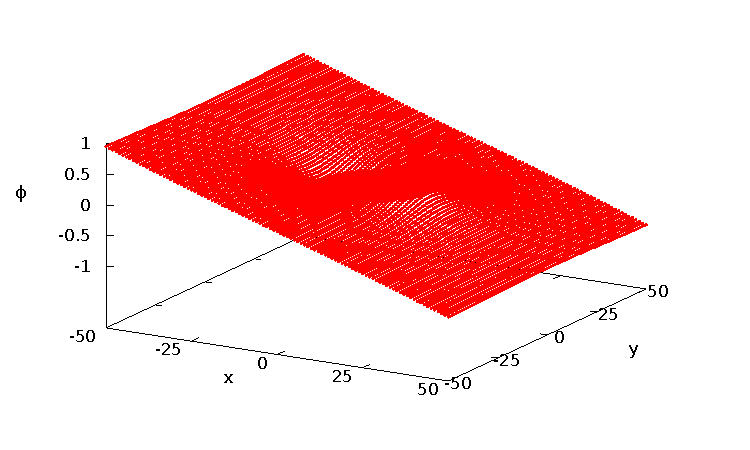
\includegraphics[scale=0.8]{analytic.pdf}
\caption{Analytic solution with $V=1$, $R=15$ on $100\times100$ grid}
\end{center}
\end{figure}

\end{frame}

\section{Numerical Solution}

\begin{frame}{Finite Difference Methods}
We approximate first derivatives as
%
\be
\frac{df}{dt} \approx \frac{f(t+\Delta t) - f(t)}{\Delta t}
\ee
%
and second derivatives as
%
\begin{align}
\frac{d^2 f}{dt^2} &\approx \frac{f'(t+\Delta t) - f'(t)}{\Delta t} \\
		   &= \frac{\frac{f(t+\Delta t) - f(t)}{\Delta t} - \frac{f(t) - f(t-\Delta t)}{\Delta t}}{\Delta t} \\
\frac{d^2 f}{dt^2} &\approx  \frac{f(t+\Delta t) - 2f(t) + f(t-\Delta t)}{\Delta t^2}
\end{align}

\end{frame}

\begin{frame}{The Relaxation Method}
Hence, Laplace's eqaution is discretised as
%
\be
\frac{\partial^2 \phi}{\partial x^2}+\frac{\partial^2 \phi}{\partial y^2} = 0
\longrightarrow
\frac{\phi_{j+1,k}-2\phi_{j,k}+\phi_{j-1,k}}{\Delta x^2} + \frac{\phi_{j,k+1}-2\phi_{j,k}+\phi_{j,k-1}}{\Delta y^2}=0
\ee
%
where $j$ and $k$ index the $x$ and $y$ directions.

For a unique step-size $\Delta = \Delta x = \Delta y$:
%
\be
\phi_{j,k}= \frac{1}{4}(\phi_{j+1,k}+\phi_{j-1,k}+\phi_{j,k+1}+\phi_{j,k-1})
\ee

The value of $\phi$ is the average of the surrounding points.
This is the relaxation method. 

\end{frame}

\begin{frame}{Algorithm}
\end{frame}

\begin{frame}{Numerical Solution}

\begin{figure}
\begin{center}
\includegraphics[scale=0.8]{potential.pdf}
\caption{Numerical potential with $V=1$, $R=15$ on $100\times100$ grid for $10000$ iterations}
\label{fig:numerical}
\end{center}
\end{figure}

\end{frame}

\section{Comparison of Analytical and Numerical Solution}

\section{Software}

\begin{frame}{Other Electrostatic Systems}
\begin{figure}
\centering
\begin{subfigure}[b]{0.45\textwidth}
	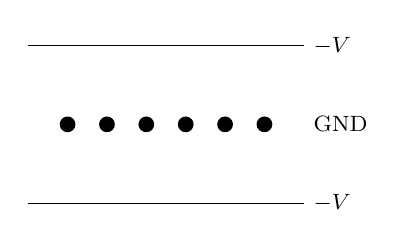
\begin{tikzpicture}
	\draw (0,0) -- (3.5,0) node[right, font=\footnotesize] {$-V$};
	\draw (0,2) -- (3.5,2) node[right, font=\footnotesize] {$-V$};
	\draw [draw=none](0,1) -- (3.5,1) node[right, font=\footnotesize] {GND};
	\fill [fill=black] (0.5,1) circle (1mm);
	\fill [fill=black] (1,1) circle (1mm);
	\fill [fill=black] (1.5,1) circle (1mm);
	\fill [fill=black] (2,1) circle (1mm);
	\fill [fill=black] (2.5,1) circle (1mm);
	\fill [fill=black] (3,1) circle (1mm);
	\end{tikzpicture}
	\caption{System B}
\end{subfigure}
\quad
\begin{subfigure}[b]{0.45\textwidth}
	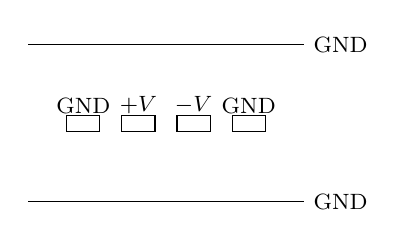
\begin{tikzpicture}
	\draw (0,0) -- (3.5,0) node[right, font=\footnotesize] {GND};
	\draw (0,2) -- (3.5,2) node[right, font=\footnotesize] {GND};
	\draw (0.49,0.9) rectangle (0.91,1.1) node[midway, above, font=\footnotesize] {GND};
	\draw (1.19,0.9) rectangle (1.61,1.1) node[midway, above, font=\footnotesize] {$+V$};
	\draw (1.89,0.9) rectangle (2.31,1.1) node[midway, above, font=\footnotesize] {$-V$};
	\draw (2.59,0.9) rectangle (3.01,1.1) node[midway, above, font=\footnotesize] {GND};
	\end{tikzpicture}
	\caption{System D}
\end{subfigure}

\begin{subfigure}[b]{0.45\textwidth}
	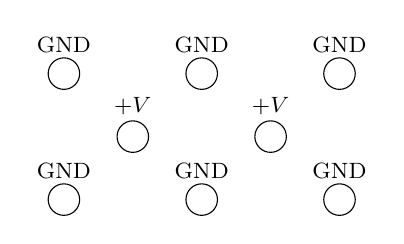
\begin{tikzpicture}
	\draw (0,0) circle (2mm) node[above, font=\footnotesize, yshift=0.15cm] {GND};
	\draw (1.75,0) circle (2mm) node[above, font=\footnotesize, yshift=0.15cm] {GND};
	\draw (3.5,0) circle (2mm) node[above, font=\footnotesize, yshift=0.15cm] {GND};
	\draw (0,1.6) circle (2mm) node[above, font=\footnotesize, yshift=0.15cm] {GND};
	\draw (1.75,1.6) circle (2mm) node[above, font=\footnotesize, yshift=0.15cm] {GND};
	\draw (3.5,1.6) circle (2mm) node[above, font=\footnotesize, yshift=0.15cm] {GND};
	\draw (0.875,0.8) circle (2mm) node[above, font=\footnotesize, yshift=0.15cm] {$+V$};
	\draw (2.625,0.8) circle (2mm) node[above, font=\footnotesize, yshift=0.15cm] {$+V$};
	\end{tikzpicture}
	\caption{System E}
\end{subfigure}
\quad
\begin{subfigure}[b]{0.45\textwidth}
	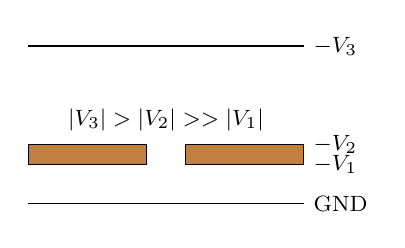
\begin{tikzpicture}
	\draw (0,0) -- (3.5,0) node[right, font=\footnotesize] {GND};
	\draw (0,2) -- (3.5,2) node[right, font=\footnotesize] {$-V_3$};
	\draw (0,0.75) -- (1.5,0.75);
	\draw (2,0.75) -- (3.5,0.75) node[right, font=\footnotesize] {$-V_2$};
	\draw (0,0.5) -- (1.5,0.5);
	\draw (2,0.5) -- (3.5,0.5) node[right, font=\footnotesize] {$-V_1$};
	\draw [fill=brown] (0,0.5) rectangle (1.5,0.75);
	\draw [fill=brown] (2,0.5) rectangle (3.5,0.75);
	\draw [draw=none] (1.75,0.8) circle (1mm) node[above, font=\footnotesize] {$|V_3|>|V_2|>>|V_1|$};
	\end{tikzpicture}
	\caption{System F}
\end{subfigure}

\caption{Alternate electrostatic configurations}
\end{figure}

\end{frame}

\begin{frame}{Software Package}
\end{frame}

\begin{frame}{Bitmaps}
\end{frame}

\begin{frame}{Boolean Mask}
\end{frame}

\begin{frame}{Convergence locking}
\end{frame}

\begin{frame}{Succesive Over Relaxation}
\end{frame}

\begin{frame}{Timing and CPU Usage}
\end{frame}

\section{Conclusion}

\begin{frame}{Conclusion}
\end{frame}

\begin{frame}
\titlepage
\end{frame}

\end{document} %end of document
